\documentclass[tikz,border=10pt]{standalone}

\begin{document}

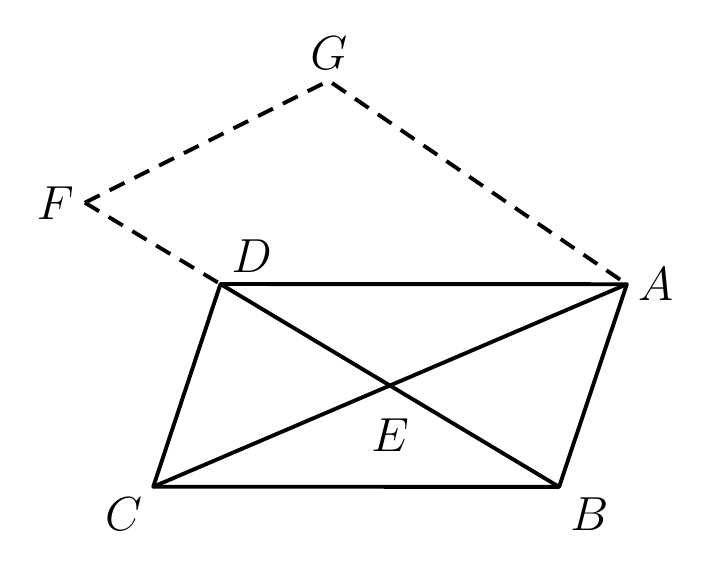
\begin{tikzpicture}[line width=1.4pt, line join=round]
\coordinate (A) at (3.439,-0.177);
\coordinate (B) at (2.579,-2.751);
\coordinate (C) at (-2.575,-2.749);
\coordinate (D) at (-1.722,-0.175);
\coordinate (E) at (0.431,-1.465);
\coordinate (F) at (-3.444,0.858);
\coordinate (G) at (-0.347,2.407);



\draw (D) -- (A) -- (B) -- (C) -- cycle;
\draw (A) -- (C);
\draw (D) -- (B);


\draw[dash pattern=on 6pt off 4pt] (F) -- (G) -- (A);
\draw[dash pattern=on 6pt off 4pt] (F) -- (D);


\node[right] at (A) {\fontsize{16}{19}\selectfont $A$};
\node[below right] at (B) {\fontsize{16}{19}\selectfont $B$};
\node[below left] at (C) {\fontsize{16}{19}\selectfont $C$};
\node[above right] at (D) {\fontsize{16}{19}\selectfont $D$};
\node[below, yshift=-8pt] at (E) {\fontsize{16}{19}\selectfont $E$};
\node[left] at (F) {\fontsize{16}{19}\selectfont $F$};
\node[above] at (G) {\fontsize{16}{19}\selectfont $G$};

\end{tikzpicture}
\end{document}